\documentclass[../2.tex]{subfiles}
\begin{document}
    Graphs can be used to encode a wide variety of data, from social networks friendships to maps.    
    We can actually consider graphs as the first topological notion introduced in mathematics.
    Their introduction dates back to the XVIII century.
    Euler noticed that in Koningsberg, there was no path that 
    allowed to cross all seven bridges just once, therefore he started to simplify the problem to approach it in a more mathematical 
    way.
    \begin{figure}[H]
        \begin{minipage}{.5\textwidth}
            \centering
            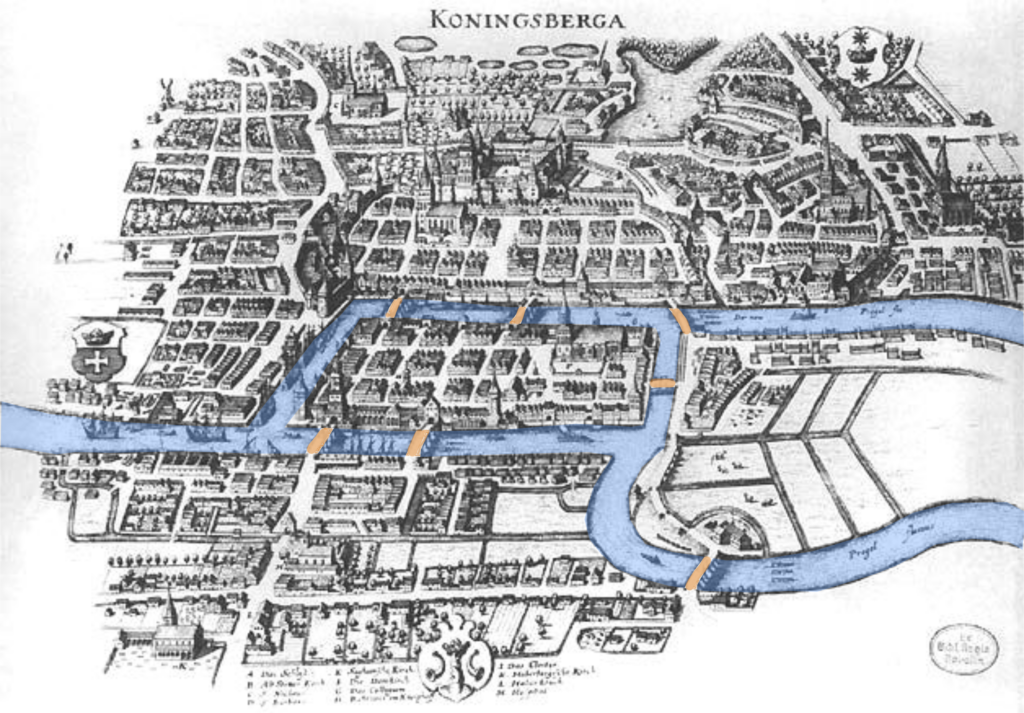
\includegraphics[width=6cm, height=4cm]{sections/2/Bridge}
            \caption{The city of Konigsberg and the\\ seven bridges.}
            \label{fig:2:1}
        \end{minipage}
        \begin{minipage}{.5\textwidth}
            \centering
            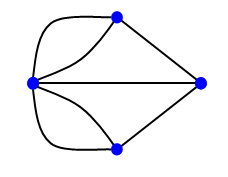
\includegraphics[width=4cm, height=3cm]{sections/2/kgraph}
            \caption{Graph representing Konigsberg's seven bridges.}
            \label{fig:2:2}
        \end{minipage}
    \end{figure}

    This led Euler to formulate an abstract approach to the problem that led to its solution, presented to the St. Petersburg
    Academy in 1735.

    In \autoref{ch:1} we presented abstract simplicial complexes, in this chapter we shall discuss in detail
    $1$-dimensional abstract simplicial complexes and how they are related to graphs.

    \begin{defn}
        An \ii{undirected graph} $\mc{G}$ is an orderd pair $(V(\mc{G}),E(\mc{G}))$, consisting of a set $V(\mc{G})$ of \ii{vertices}
        and a set $E(\mc{G})$, disjoint from $V(\mc{G})$, of \ii{edges}, together with an incidence function
        $\psi_\mc{G}:E(\mc{G}) \to V(\mc{G}) \times V(\mc{G})$ that associates with each edge of G an unordered pair of (not necessarily
        distinct) vertices of $\mc{G}$. If $e$ is an edge and $u$ and $v$ are vertices such that $\psi_\mc{G}(e) =
        \{u, v\}$, then $e$ is said to \ii{join} $u$ and $v$, and the vertices $u$ and $v$ are called the \ii{ends}
        of $e$. A graph where the ordering of the ends of an edge is meaningful is said to be a \ii{directed} graph.
    \end{defn}

    \begin{defn}
        Let $\mc{G}$ be a graph, we define the \ii{adjacency matrix} $A$ of $\mc{G}$ by
        \[a_{ij} = 
        \begin{cases}
            1 & \exists e \in E(\mc{G}) : \psi_\mc{G}(e) = \{i,j\} \\
            0 & otherwise \\
        \end{cases}. \]        
    \end{defn}

    \begin{defn}
        A graph is \ii{simple} if it has no loops nor parallel edges, i.e. there is a unique edge joining two different vertices.
    \end{defn}
    
    Much of graph theory is concerned with the study of simple graphs.

    \begin{prop}
        A \ii{simple undirected graph} $\mc{G}$ is representable with $1$-dimensional abstract simplicial complex.
    \end{prop}
    \begin{proof}
        Let's construct a family of sets $\mc{A}$ in the following way.
        \[ \mc{A} = V(\mc{G}) \cup \{ \{i,j\} \in V(\mc{G}) \times V(\mc{G}) : \exists e \in E(\mc{G}) \quad \psi_\mc{G}(e)=\{i,j\}\}. \]
        It is easy to see that this is an abstract simplicial complex of dimension $1$.
    \end{proof}

    % In a graph $\mc{G}$ the non trivial chain groups are therefore $C_0(\mc{G})$ and $C_1(\mc{G})$, also called vertex and edge spaces. 
    % The canonical basis of the vertex space is the set of vertexes $\{\ket{i}\}_{i \in I}$, and that of edges which is a subset of $\{\ket{i,j}\}_{(i,j)\in I\times I}$.

    \begin{defn}
        Let $\mc{G}$ be a simple undirected graph, we define the \ii{adjacency matrix} $A$ of $\mc{G}$ on the canonical vertex basis by
        \[a_{ij} = 
        \begin{cases}
            1 & \ket{i,j} \in C_1 \\
            0 & otherwise \\
        \end{cases}. \]        
    \end{defn}

    Since $C_1$ is a group, whenever $\ket{i,j} \in C_1$ then also $\ket{j,i} = -\ket{i,j} \in C_1$. In order to represent simple directed
    graphs we need to choose a canonical basis $B_1$ of oriented $p$-simplices.

    \begin{defn}
        Let $\mc{G}$ be a simple directed graph w.r.t. $B_1$, we define the \ii{adjacency matrix} $A$ of $\mc{G}$ on the canonical vertex basis by
        \[a_{ij} = 
        \begin{cases}
            1 & \ket{i,j} \in B_1 \\
            0 & otherwise \\
        \end{cases}. \]  
    \end{defn}

\end{document}